\documentclass{beamer}
\usepackage{beamerthemeshadow}
\usepackage{color}
%\usepackage[all]{xy}

%\newcommand{\comment}[1]{}
\newcommand{\comment}[1]{{\bf \tt  {#1}}}
\definecolor{ForestGreen}{RGB}{34,139,34}
\newcommand{\emcomment}[1]{\textcolor{ForestGreen}{\comment{Elena: {#1}}}}
\newcommand{\todo}[1]{\textcolor{blue}{\comment{To Do: {#1}}}}
\newcommand{\pscomment}[1]{\textcolor{red}{\comment{Paul: {#1}}}}
\newcommand{\mmcomment}[1]{\textcolor{magenta}{\comment{Max: {#1}}}}

\mode<presentation>
{
  \usetheme{Copenhagen} %%% Change later
 \usecolortheme{beaver}


  \setbeamercovered{transparent}
  % or whatever (possibly just delete it)
}
\setbeamertemplate{footline}[page number]{}


\begin{document}
\title{Developing a Graphical Library for a Clojure-based Introductory CS Course}
\author{Paul Schliep, Max Magnuson, Elena Machkasova}
\institute[UMM] % (optional, but mostly needed)
{
  Midwest Instruction and Computing Symposium
  
  University of Minnesota, Morris
}
\date{April 25, 2014}

\begin{frame}
  \titlepage
\end{frame}

\begin{frame}

  \frametitle{Outline}
\tableofcontents

\end{frame}

\section{Introduction to the project}

\begin{frame}
\frametitle{The Project}
\begin{itemize}
\item Contributing to ClojureEd on adapting to Clojure for an introductory course
\item Objective is to develop a graphical library for Clojure
\item We hope this graphical library can be useful for the introductory course
\item Work in progress
\end{itemize}
\end{frame}

\begin{frame}
\frametitle{Introduction to Clojure}
\begin{itemize}
\item Developed by Rich Hickey in 2007
\item Functional programming language in the Lisp family
\item Runs on the JVM
\item Immutable data structures and first class functions
\item Data structures such as lists, vectors, hashmaps
\end{itemize}
\end{frame}

\begin{frame}
\frametitle{UMM's introductory CS course}
\begin{itemize}
\item Students are not expected to have prior programming knowledge
\item The course currently utilizes Racket to help teach key concepts
\item Racket is a functional language similar to Clojure
\item Functional languages help students learn concepts like recursion and higher order functions
\item The course makes use of Racket's graphical library 
\end{itemize}
\end{frame}

\begin{frame}
\frametitle{Racket graphical library game example}
\begin{center}
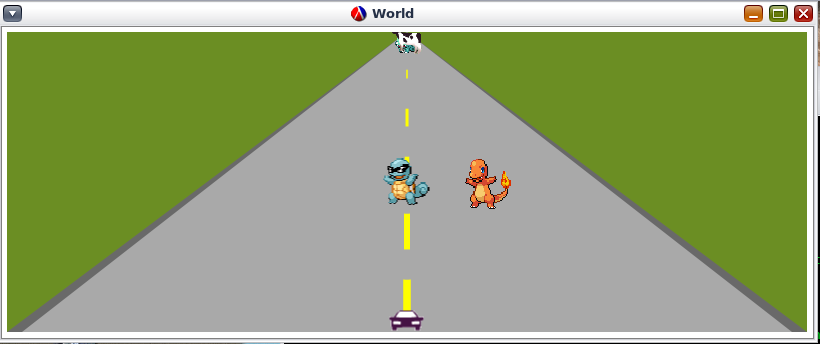
\includegraphics[width=300pt]{racketGameExample}
\end{center}
\end{frame}

\begin{frame}
\frametitle{Benefits and limitations of Clojure}
Benefits:
\begin{itemize}
\item Gaining traction in the industry
\item Offers better parallel processing
\item Integration with Java
\end{itemize}
Limitations:
\begin{itemize}
\item Unintuitive error messages
\item Lacks a graphical library
\item Lack of an IDE suitable for beginner CS students
\end{itemize}
\end{frame}

\begin{frame}[fragile]
\frametitle{Clojure Syntax}
\begin{itemize}
	\item Prefix notation			
	\begin{verbatim}
		(<name of function> <argument 1> <argument 2> ...)
		(+ 2 2)
		-> 4
	\end{verbatim}
	\item Defn
	\begin{verbatim}
		(defn square[x] (* x x))
	\end{verbatim}
	\item Anonymous functions
	\begin{verbatim}
		(fn [x] (* x x))
	\end{verbatim}
	\item First class functions
	\begin{verbatim}
		(map square [1 2 3 4])
		-> [1 4 9 16]
	\end{verbatim}
	\item Hashmaps
	\begin{verbatim}
	 	{:a 1 :b 2 :c 3}
	\end{verbatim}
\end{itemize}
\end{frame}

\section{Goals and setup for an introductory course}

\begin{frame}
\frametitle{Introduction to functional approaches}
\begin{itemize}
\item Stylistic choice for programming
\item Immutable data types
\item Less dependency on order
\item First class functions
\end{itemize}
\end{frame}

\begin{frame}
\frametitle{Requirements for a graphical library}
\begin{itemize}
\item Reinforce functional approaches from Clojure
\item Accessible to introductory students
\item Implement Model-view-controller (MVC) similar to Racket's graphical library
	\begin{itemize}
	\item Checkers example
	\end{itemize}
\end{itemize}
\begin{center}
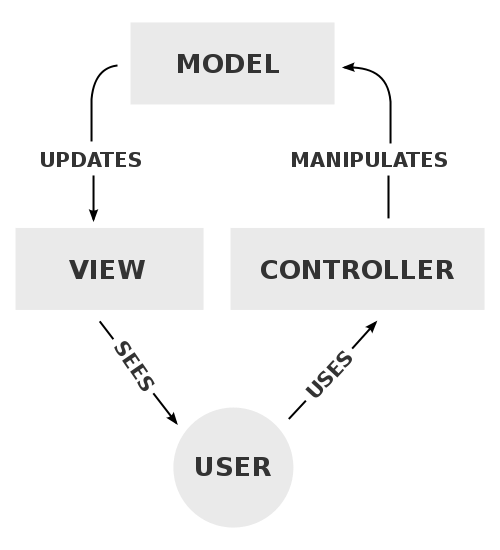
\includegraphics[width=100pt]{MVC-Process}
\end{center}
%\pscomment{Add graphic for MVC}
\end{frame}

\section{Developing a Clojure graphical library}

\begin{frame}
\frametitle{Overview of Quil}
\begin{itemize}
\item Open source graphical library for Clojure
\item Provides functionality suitable for introductory-level projects
\item Built on top of Java Swing
\item Continuously being developed
\end{itemize}
\end{frame}

\begin{frame}[fragile]
\frametitle{Developing programs with Quil}
\begin{itemize}
\item Defsketch
\item Works using frames and frame rate
\item Draws in layers
\item Supports input from keyboard and mouse
\begin{verbatim}
(defsketch example 
:title "Example"
:setup setup-example
:draw draw-example
:size [400 300])
\end{verbatim}
\end{itemize}
\end{frame}

\begin{frame}[fragile]
\frametitle{Example of a Quil program}
  \begin{columns}[T]
    \begin{column}{.5\textwidth}
      \begin{block}{Example Code:}
        \begin{verbatim}
(defn setup-example []
(frame-rate 1)
(background 200))

(defn draw-example []
(ellipse
(random (width))
(random (height))
100 100))
        \end{verbatim}
      \end{block}
    \end{column}

    \begin{column}{.5\textwidth}
      \begin{block}{Our Image}
        \begin{center}
        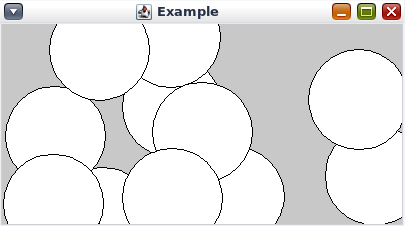
\includegraphics[width=150pt]{quil-example}
        \end{center}
      \end{block}
    \end{column}
  \end{columns}

\end{frame}

\begin{frame}
\frametitle{Issues with Quil}
\begin{itemize}
\item Imperative approaches
	\begin{itemize}
		\item Often requires direct manipulation of state
		\item Dependencies on order
		\item Inconsistent with introductory course goals
	\end{itemize}
\item Underdocumented API
\end{itemize}
\end{frame}

\section{Our graphical library}

\begin{frame}
\frametitle{Development of the graphical library}
\begin{itemize}
\item Abstracted over Quil's functions
	\begin{itemize}
	\item Defsketch
	\item Shapes
	\item Colors
	\item Text
	\end{itemize}
\item Handling state in a functional approach
	\begin{itemize}
		\item Models MVC
	\end{itemize}
\end{itemize}
\end{frame}


\begin{frame}
\frametitle{How our graphical library works}
\begin{itemize}
\item Separates handling of state
	\begin{itemize}
	\item MVC
	\item update
	\item display
	\end{itemize}
\end{itemize}
\end{frame}

\begin{frame} [fragile]
\frametitle{An example made using our graphical library}
\begin{verbatim}
(def states
{:snake [450 450 450 470 450 490 450 510], 
:snake-head [450 450], 
:food [150 150], 
:snake-direction "north", :score 0})

(def updates
{:setup-drawing setup 
:snake update-snake
:food update-food})

(def display-order
[draw-canvas draw-food draw-snake])
\end{verbatim}
%\todo{snake screenshot}
\end{frame}

\begin{frame}
\frametitle{Snake Example}
\begin{center}
\fbox{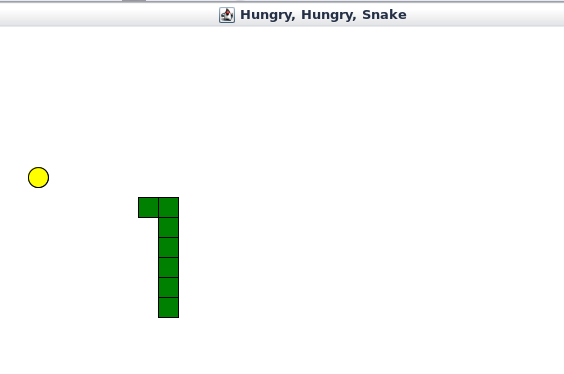
\includegraphics[width=200pt]{snake}}
\end{center}
\end{frame}

\begin{frame}
\frametitle{Differences in handling state in Racket}
\begin{columns}[T]
\begin{column}{.95\textwidth}
\begin{block}{Racket gives entire state to user}
\begin{center}
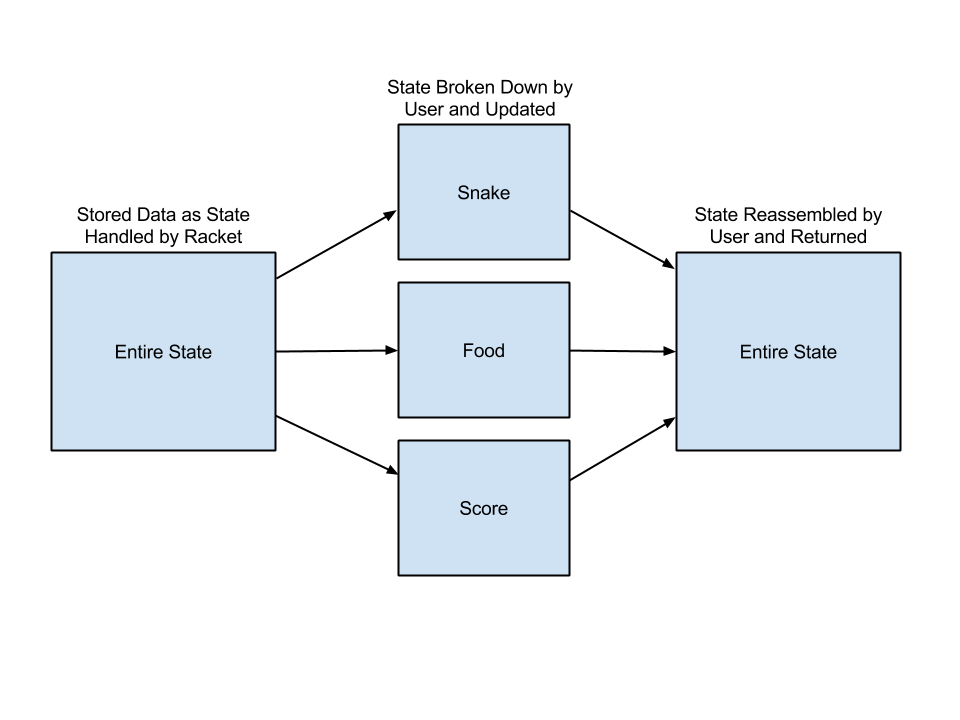
\includegraphics[width=270pt]{Rackets_State_Diagram}
\end{center}
\end{block}
\end{column}
\end{columns}
\end{frame}

\begin{frame}
\frametitle{Diagram of handling state in our graphical library}
\begin{columns}[T]
\begin{column}{.95\textwidth}
\begin{block}{Our system breaks state down for the user}
\begin{center}
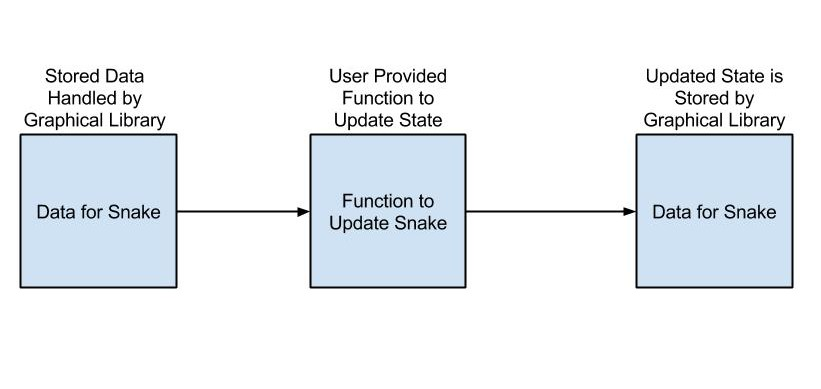
\includegraphics[width=240pt]{Handling_State_in_Graphical_Library}
\end{center}
\end{block}
\end{column}
\end{columns}
\end{frame}

\section{Conclusions and future work}

\begin{frame}
\frametitle{Conclusions}
\begin{itemize}
\item Good start for abstracting over Quil's functions
\item More functional approach
\item Graphical library shows promise
\end{itemize}
\end{frame}

\begin{frame}
\frametitle{Future Work}
\begin{itemize}
\item This is still work in progress
\item Create our own macro to abstract over defsketch
\item Abstract over more functions in Quil
\item Develop an API with examples for students
\end{itemize}
\end{frame}

\begin{frame}
\frametitle{Selected references}
Selected references:
\begin{itemize}
\item Quil https://github.com/quil/quil
\item Filleisen, M., Findler, R. B., Flatt, M. and Krishnamurthi, S. How to design programs: an introduction to programming and computing. MIT Press, Cambridge, MA, USA 2001.
\item Hickey, R. The clojure programming language. In Proceedings of the 2008 symposium on Dynamic languages(New York,NY,USA,2008),DLS'08,ACM,pp.1:1-1:1.
\end{itemize}
\end{frame}

\begin{frame}
\frametitle{Acknowledgements}
The authors would like to thank
\begin{itemize}
\item Nick Skube and Niccolas Ricci
\item Developers of Quil
\item Friends and Family
\end{itemize}
\end{frame}


\end{document}
